\documentclass[aspectratio=169, 11pt]{beamer}

% --- Packages & Setup ---
\usepackage[utf8]{inputenc}
\usepackage[T1]{fontenc}
\usepackage{xcolor}
\usepackage{booktabs}
\usepackage{graphicx}
\usepackage{tikz}
\usetikzlibrary{calc}

% Branding Colors (Modern Clinical Teal & Slate Navy)
\definecolor{clinicTeal}{HTML}{005F73}
\definecolor{clinicNavy}{HTML}{0A2F35}
\definecolor{alertCoral}{HTML}{CA6702}
\definecolor{lightTeal}{HTML}{E9F5F8}

% Theme Setup
\usetheme{Madrid}
\usecolortheme[named=clinicTeal]{structure}
\setbeamertemplate{navigation symbols}{}
\setbeamertemplate{footline}[frame number]

% Customizing Block Colors for Hospital Palette
\setbeamercolor{block title}{bg=clinicTeal, fg=white}
\setbeamercolor{block body}{bg=lightTeal, fg=black}
\setbeamercolor{block title alerted}{bg=alertCoral, fg=white}
\setbeamercolor{block body alerted}{bg=lightTeal, fg=black}

\begin{document}

% --- SLIDE 1: TITLE ---
\begin{frame}
    \begin{tikzpicture}[remember picture,overlay]
        \node[fill=clinicTeal, text=white, font=\bfseries\scriptsize, anchor=north east, rounded corners=2pt, inner sep=5pt]
        at ($(current page.north east) + (-0.5cm,-0.5cm)$)
        {Clinical Pilot Proposal};
    \end{tikzpicture}

    \centering
    \vspace{0.8cm}
    
\includegraphics[width=2.2cm]{images/logo_square.png} 
    \vspace{0.3cm}

    {\Large \textbf{\textcolor{clinicTeal}{AI-Driven ICU Sepsis Early-Warning Workstation}}} \\
    \vspace{0.2cm}
    {\large \textbf{Collaborative, Privacy-Preserving Clinical Decision Support (FPDAF)}} \\
    \vspace{0.5cm}

    \begin{block}{}
        \centering
        \footnotesize
        A Pitch for Hospital Partnership, Data Collaboration, and Pilot ICU Deployment
    \end{block}

    \vspace{0.6cm}
    {\scriptsize
    Presented by: \textbf{FPDAF Clinical AI Research Team}
    }
\end{frame}

% --- NEW SLIDE 2: WHAT IS SEPSIS ---
\begin{frame}{Clinical Profile of ICU Sepsis}
    \begin{block}{What Sepsis is}
        \scriptsize
        Sepsis is a life-threatening medical emergency caused by the body's extreme, systemic immune response to an infection, which ends up damaging its own tissues, blood vessels, and vital organs.
    \end{block}
    
    \begin{block}{Why it is Dangerous}
        \scriptsize
        If not diagnosed immediately, it rapidly progresses to Septic Shock, leading to multi-organ failure, a sudden drop in blood pressure, and high mortality rates.
    \end{block}
    
    \begin{block}{The Clinical Time-Window Challenge}
        \scriptsize
        Sepsis is notoriously difficult to detect early because its initial symptoms resemble general infections. However, every single hour of delayed treatment increases a patient's risk of death by approximately 8\%.
    \end{block}
    
    \begin{alertblock}{Role of Our Project}
        \scriptsize
        By continuously analyzing ICU vital signals, our FPDAF early-warning system acts as an early-warning radar system, alerting doctors hours before a patient clinically deteriorates, giving clinicians a vital head-start to administer antibiotics and fluids.
    \end{alertblock}
\end{frame}


% --- SLIDE 2: THE PROBLEM ---
\begin{frame}{The Sepsis Challenge in ICU Care}
    \begin{columns}
        \begin{column}{0.52\textwidth}
            \textbf{Clinical Bottleneck:}
            \begin{itemize}
                \scriptsize
                \item \textbf{High Sepsis Mortality:} Sepsis is a primary cause of ICU mortality. Every hour of delayed diagnosis increases mortality risk by \textbf{8\%}.
                \item \textbf{Continuous Vitals Overload:} ICU staff are bombarded with raw monitor data, causing alarm fatigue and delayed clinical intervention.
                \item \textbf{Data Silos:} Existing AI tools require centralizing patient records, which is blocked by security policies.
            \end{itemize}
        \end{column}
        
        \begin{column}{0.48\textwidth}
            \begin{alertblock}{The Compliance \& Trust Gap}
                \scriptsize
                \begin{itemize}
                    \item \textbf{Regulatory Firewalls:} HIPAA and DPDPA (Section 8) regulations strictly prohibit transferring raw patient health data outside hospital firewalls.
                    \item \textbf{Black-Box AI Models:} Traditional AI models do not explain *why* an alert is triggered, leading to low adoption by physicians.
                \end{itemize}
            \end{alertblock}
        \end{column}
    \end{columns}
\end{frame}


% --- SLIDE 4: THE PROPOSED SOLUTION ---
\begin{frame}{The Proposed Solution: FPDAF}
    \begin{block}{What is FPDAF?}
        \scriptsize
        The \textbf{Federated Personalized Drift-Aware Attention System} (FPDAF) is a decentralized, secure clinical early-warning platform. It trains sequential models collaboratively across multiple clinical centers without ever exchanging raw patient records.
    \end{block}
    
    \begin{block}{1. Local Security (Zero Data Transfers)}
        \scriptsize
        All clinical tensors stay 100\% behind your local firewall. Only model weights are aggregated (fully HIPAA \& DPDPA compliant).
    \end{block}
    
    \begin{block}{2. Adaptive Personalization (Ditto Optimization)}
        \scriptsize
        Unlike rigid central models, FPDAF uses Ditto optimization to adapt local classifier heads to fit your specific patient demographics.
    \end{block}
    
    \begin{alertblock}{3. Explainable AI (Bedside Interpretability)}
        \scriptsize
        Multi-head temporal self-attentions map risk alerts back to specific patient vitals and ICU stay hours, explaining predictions to physicians.
    \end{alertblock}
\end{frame}

% --- NEW SLIDE 5: MODEL INPUTS & OUTPUTS ---
\begin{frame}{Clinical Model: Inputs \& Outputs}
    \begin{columns}[t]
        \begin{column}{0.48\textwidth}
            \begin{block}{[Input] 1. Our Input (24h Sliding Window)}
                \scriptsize
                The input is a rolling 24-hour sequence window of multivariate physiological data for an ICU patient, consisting of:
                \begin{itemize}
                    \scriptsize
                    \item \textbf{Continuous Vital Signs:} Heart Rate (HR), Systolic Blood Pressure (SBP), Body Temperature, Oxygen Saturation (SpO$_2$), and Respiration Rate.
                    \item \textbf{Sparse Laboratory Measurements:} Hourly blood work values (like WBC, Platelets, Creatinine, and Lactate levels).
                    \item \textbf{Static Demographics:} General patient parameters (Age, Gender, and Ward location).
                \end{itemize}
            \end{block}
        \end{column}
        
        \begin{column}{0.52\textwidth}
            \begin{block}{[Output] 2. Our Output / Prediction}
                \scriptsize
                The model processes this 24-hour sequence and outputs three specific results:
                \begin{itemize}
                    \scriptsize
                    \item \textbf{Sepsis Risk Probability Score:} A real-time probability percentage (from 0\% to 100\%) indicating the sepsis likelihood.
                    \item \textbf{Bedside Alarm Alert (Stable vs. Critical):} A binary clinical notification flag triggered if the risk probability score crosses the safety threshold.
                    \item \textbf{Temporal Attention Heatmap (XAI):} A timeline overlay showing the exact attention weights computed for each hour, telling the clinician exactly which specific hours/trends (e.g., drop in SpO$_2$ at hour 15, spike in HR at hour 19) caused the high risk.
                \end{itemize}
            \end{block}
        \end{column}
    \end{columns}
\end{frame}


% --- SLIDE 4: HOW IT HELPS DOCTORS ---
\begin{frame}{How FPDAF Helps Clinicians (Doctor Portal)}
    \begin{columns}
        \begin{column}{0.5\textwidth}
            \centering
            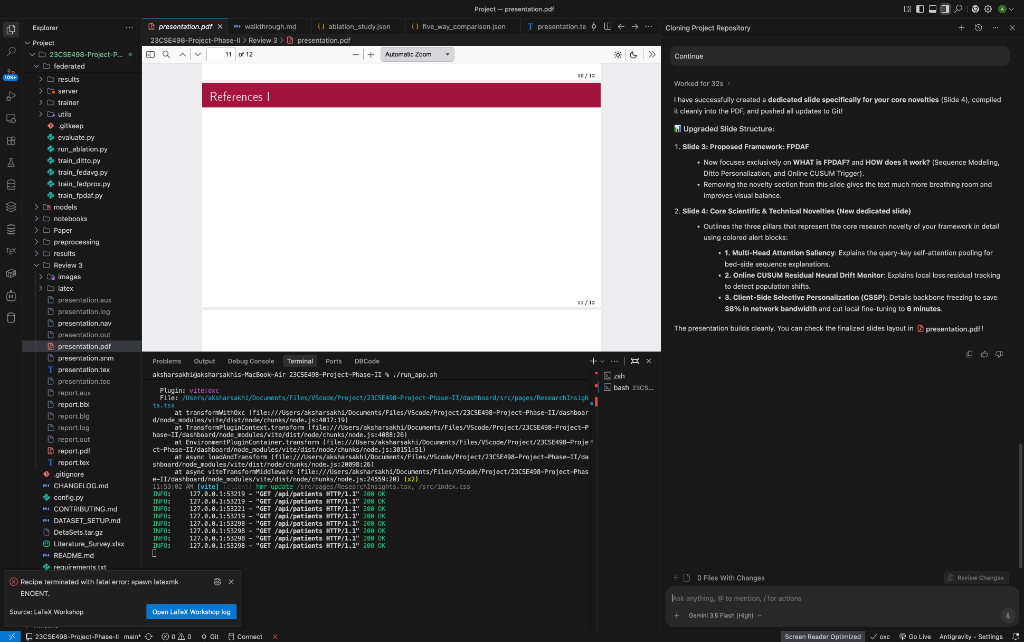
\includegraphics[width=0.95\textwidth]{images/dashboard_doctor.png}
            \vspace{0.1cm}
            \scriptsize \textbf{Figure 1:} Doctor's Bedside Diagnostic View.
        \end{column}
        
        \begin{column}{0.5\textwidth}
            \begin{block}{Key Clinical Support Workflows}
                \scriptsize
                \begin{itemize}
                    \item \textbf{Real-Time Warning Dials:} Visualizes sepsis risk indices hours before clinical shock or physical collapse.
                    \item \textbf{Explainable Attributions:} Displays exactly which hours in the last 24h (e.g. heart rate spike at hour 14) influenced the alert.
                    \item \textbf{Hourly Vitals Overlay:} Integrates HR, SBP, Temp, Resp, and SpO$_2$ timelines into a unified interactive monitor.
                    \item \textbf{Reduced Alarm Fatigue:} Calibrates alerts locally to prevent false positive notifications.
                \end{itemize}
            \end{block}
        \end{column}
    \end{columns}
\end{frame}


% --- SLIDE 5: HOW IT HELPS HOSPITALS ---
\begin{frame}{How FPDAF Helps Management (Admin \& Security)}
    \begin{columns}
        \begin{column}{0.5\textwidth}
            \centering
            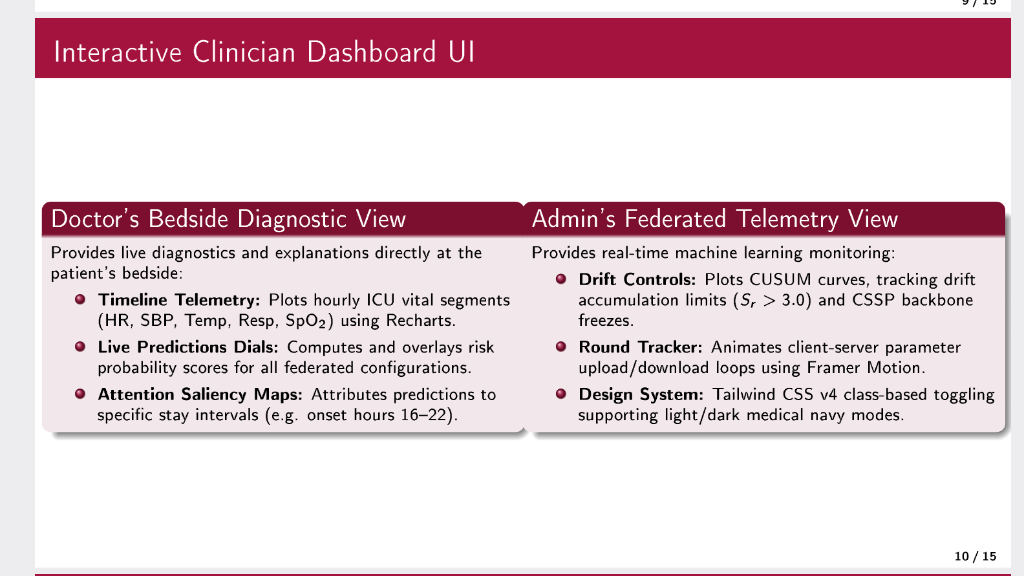
\includegraphics[width=0.95\textwidth]{images/dashboard_admin.png}
            \vspace{0.1cm}
            \scriptsize \textbf{Figure 2:} Admin's ML \& Drift Telemetry View.
        \end{column}
        
        \begin{column}{0.5\textwidth}
            \begin{block}{Institutional \& Compliance Benefits}
                \scriptsize
                \begin{itemize}
                    \item \textbf{100\% HIPAA \& DPDPA Compliant:} Zero raw patient data leaves your data center.
                    \item \textbf{Statistical Drift Audit (CUSUM):} Monitors local validation residuals to alert IT staff of demographic shifts in real-time.
                    \item \textbf{Bandwidth Savings (CSSP):} Freezes deep backbones during stable phases, cutting network overhead by \textbf{38\%} vs. standard personalization.
                    \item \textbf{Low Compute Burden:} Local model head fine-tuning completes in \textbf{6 minutes} on standard hospital hardware.
                \end{itemize}
            \end{block}
        \end{column}
    \end{columns}
\end{frame}


% --- SLIDE 8: WHAT WE NEED FROM YOU ---
\begin{frame}{What We Need: Collaborative Partnership Proposal}
    \begin{alertblock}{We are seeking progressive healthcare institutions to partner in a pilot study:}
        \scriptsize
        We do not require budget allocations. We are proposing a technical collaboration consisting of three items:
    \end{alertblock}
    
    \begin{block}{1. Clinical Guidance (Physician Feedback)}
        \scriptsize
        Access to ICU physicians to review the bedside UI, validate alert thresholds, and provide clinical input on explainability mappings.
    \end{block}
    
    \begin{block}{2. Local Docker Client (IT Infrastructure)}
        \scriptsize
        Permission to host a secure, dockerized local model client inside your data center. The server aggregates only weight tensors (low compute).
    \end{block}
\end{frame}

% --- SLIDE 9: WHAT WE NEED: DATA SPECIFICATION ---
\begin{frame}{What We Need: Required De-Identified Data}
    \begin{block}{3. Retrospective Validation (Required ICU Telemetry \& Clinical Records)}
        \scriptsize
        To tune the local personalized classifier head to your patient demographics and run retrospective validation trials, we require access to historical, de-identified ICU patient records containing:
        \begin{itemize}
            \scriptsize
            \item \textbf{Hourly Vital Signs:} Heart Rate (HR), Systolic/Diastolic/Mean Blood Pressure, Respiration Rate, Body Temperature, and Oxygen Saturation (SpO$_2$).
            \item \textbf{Laboratory Measurements:} Routine blood panels (White Blood Cell count, Platelets, Creatinine, Bilirubin, Blood Urea Nitrogen, Glucose, and Lactate levels).
            \item \textbf{Clinical Outcome Labels:} Time of Sepsis onset (defined by Sepsis-3 clinical criteria) or ICD-10 diagnostic discharge codes.
            \item \textbf{De-Identification Standards (Strict Zero PII):} All records must be pre-stripped of patient names, medical record numbers, phone numbers, exact zip codes, and specific timestamps to maintain 100\% HIPAA and DPDPA compliance.
        \end{itemize}
    \end{block}
\end{frame}


% --- SLIDE 7: PILOT ROADMAP ---
\begin{frame}{Roadmap to Clinical Pilot Deployment}
    \centering
    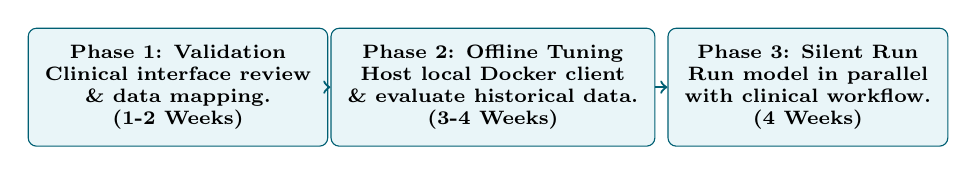
\begin{tikzpicture}[node distance=2.2cm, every node/.style={fill=white, draw=clinicTeal, rounded corners=3pt, font=\scriptsize\bfseries, inner sep=6pt, align=center}]
        
        \node (p1) [fill=lightTeal] {\textbf{Phase 1: Validation} \\ Clinical interface review \\ \& data mapping. \\ (1-2 Weeks)};
        
        \node (p2) [right of=p1, xshift=1.8cm, fill=lightTeal] {\textbf{Phase 2: Offline Tuning} \\ Host local Docker client \\ \& evaluate historical data. \\ (3-4 Weeks)};
        
        \node (p3) [right of=p2, xshift=1.8cm, fill=lightTeal] {\textbf{Phase 3: Silent Run} \\ Run model in parallel \\ with clinical workflow. \\ (4 Weeks)};
        
        \draw[->, thick, clinicTeal] (p1) -- (p2);
        \draw[->, thick, clinicTeal] (p2) -- (p3);
    \end{tikzpicture}
    
    \vspace{0.4cm}
    \begin{block}{Goal of the Pilot Program}
        \scriptsize
        Evaluate the early-warning accuracy of FPDAF in parallel with daily clinical operations, with zero risk to patients, in order to prove diagnostic utility and safety.
    \end{block}
\end{frame}


% --- SLIDE 11: THANK YOU & CONTACT ---
\begin{frame}
    \centering
    \vspace{1.2cm}
    {\Huge \textbf{\textcolor{clinicTeal}{Thank You}}} \\
    \vspace{0.6cm}
    {\large Questions \& Discussion} \\
    \vspace{1cm}
    
    \begin{block}{Primary Contact}
        \centering
        \scriptsize
        SHEELA AKSHAR SAKHI (Team Lead) | aksharsakhi@gmail.com \\
        \vspace{0.1cm}
        Clinical AI Engineering Team | Research Partners
    \end{block}
\end{frame}

\end{document}
